% TEX-root = ../main.tex
\chapter{\LaTeX{} 模板使用指南}

\section{环境配置}
\begin{enumerate}
    \item 本地环境\\
    下载安装最新版 TexLive 或 MikTeX。
    \item 在线环境\\
    Overleaf。
\end{enumerate}

\section{编辑文件}
\begin{enumerate}
    \item \texttt{sysusetup.tex}: 填写标题、作者、导师、学位名称等信息。
    \item \texttt{data/abstract.tex}: 填写中英文摘要。
    \item \texttt{data/denotation.tex}: 填写符号与缩略语,注意按音序排序。
    \item \texttt{data/chapxx.tex}: 各章内容,如有章节增删请在\texttt{main.tex}中修改相关记录。
    \item \texttt{data/appendix.tex}: 附录。
    \item \texttt{data/works.tex}: 学术成果。
    \item \texttt{data/acknowledgements.tex}: 致谢。
    \item \texttt{ref/refs.bib}: 引文数据库。
    \item \texttt{main.tex}: 主文件,用于控制文档选项(字体,学位类别):
    \begin{enumerate}
        \item 学术硕士: \verb|\documentclass[degree=master]{sysuthesis}|;
        \item 专业硕士: \verb|\documentclass[degree=master,degree-type=professional]{sysuthesis}|;
        \item 博士: \verb|\documentclass[degree=doctor]{sysuthesis}|。
    \end{enumerate}
    指定论文要包括的部分,如摘要、目录、正文各章节、附录、引文数据库等等。
    (注意插入每章内容之后要加 \verb|\cleardoublepage| 以保证在打印版中各章都从右边开始):
    \begin{verbatim}
    % !TeX root = ../main.tex

\chapter{学位论文形式结构}

\section{字数要求}
\begin{enumerate}
    \item 硕士论文: 正文一般为$1 \sim 3$万字;
    \item 博士论文: 正文一般不超过$15$万字。
\end{enumerate}

\section{论文结构}
\begin{figure}
    \centering
    \includegraphics[width=.7\textwidth]{doc_structure.jpg}
    \caption{文档结构}
\end{figure}

\section{前置部分}

\begin{enumerate}
    \item 封面和封底:由研究生院统一印刷,封面内容一律打印,其中导师姓名以研究生院备案名单为准。\\
          题目:在25字以内,能简明、具体、确切地表达论文特定内容,必要时,可以使用副标题。中文、英文题目应一致。
      \item 扉页内容包括学位论文中文、英文题目、专业名称、申请人姓名、导师姓名及论文答辩委员会组成 (由答辩委员会成员签名)。
      \item 原创性及学位论文使用授权声明。
      \item 中英文摘要。
\end{enumerate}


\section{主体部分}
\begin{enumerate}
    \item 主体部分包括引言 (前言),国内外文献综述,正文, 结语,参考文献。要求图表清晰,叙述流畅,章节有序,层次 分明。\\
    引言 (前言)部分内容主要为本研究课题的学术背景及理论与实际意义;本研究课题的来源及主要研究内容;建立研究的线索与思路。

    \item 文中的图、表、公式等,一律用阿拉伯数字按章顺序编号。如图 1-1、图2-2, 表 1-1、表 2-1,公式 (1-1) 等。图序及图名置于图的下方,居中排列;表序及表名置于表的上方,居中排列。详见第\ref{figures_tables}章的说明。

    \item 参考文献
    \begin{enumerate}
        \item 参考文献为论文中所有引文、引用观点以及对论文有重要影响和启发的文献;
        \item 参考文献按在论文中出现的先后依次排序;个别学科若通用该学科惯用的排序规范,可以例外;
        \item 参考文献内容一般排列在论文末尾 (论文篇幅较大且引用文献较多的,可在每章末尾注出),序码与论文加注处对应;
        \item 参考文献标注格式: 使用国标GB/T 7714-2015标准, 建议使用工具自动控制引文格式, 
        以保证格式规范。
        该\LaTeX{}模板已经对引文格式做了配置,
        用户需要将所需参考文献的信息存在 \texttt{bib} 格式的文件\texttt{ref/refs.bib}中, 
        通过 \verb|\cite{}|命令在恰当位置引用 (详见第\ref{citations}章的说明)。
        \texttt{bib}文件可从文献管理工具导出或自己用 \texttt{JabRef} 等软件编辑。
    \end{enumerate}

    \item 注释:可以用 “脚注”或 “文后注”来标注引用著作中的一些观点和案例,但全文标注方式应统一。
\end{enumerate}

\section{附录部分}
\begin{enumerate}
    \item 附录\\
        附录是正文主体的补充。下列内容可以作为附录:
        \begin{enumerate}
            \item 攻读学位期间发表的 (含已录用,并有录用通知书的)与学位论文相关的学术论文目录 。
            \item 由于篇幅过大,或取材于复制件不便编入正文的材料、数据。
            \item 对本专业同行有参考价值,但一般读者不必阅读的材料。
            \item 论文中使用的符号意义、单位缩写、程序全文及有关说明书。
            \item 附件:计算机程序清单、软磁盘、鉴定证书、获奖 奖状或专利证书的复印件等。
        \end{enumerate}
    \item 后记\\
        后记是有关本论文情况的说明性文字,主要是交代编写过程,阐述作者的感想和体会,对有关单位或个人的致谢语等。
\end{enumerate} 


    \cleardoublepage
    % !TeX root = ../main.tex

\chapter{结构排版及字体规范}
\section{论文印制规格}
学位论文一律采用 A4纸张双面打印,纸的四周留足空白边缘,以便装订、复制和读者批注。

\section{中英文摘要}
硕士学位论文摘要一般不超过1200字, 博士学位论文一般不超过2000字。
关键词三到五个,用逗号分隔。

\section{目录页}
\begin{enumerate}
    \item 目录应两端对齐;
    \item 目录页排版只排到二级标题, 即章和节。
\end{enumerate}

\subsection{测试目录}
三级标题 \verb|\subsection{}| 不应出现在目录当中。

\section{主体部分}
\begin{enumerate}
    \item 章的标题应局中, 采用小二号黑体; 节的标题左边空两格, 小三号宋体, 加粗。 文章段落内容采用小四号宋体。
    \item 章与节的题目之间空两行。
    \item 节标题与段落内容之间空一行。
    \item 关于关使用文字、数字的书写法:
        \begin{enumerate}
            \item 应用汉语简化字书写。
            \item 世纪、年份一概用阿拉伯数字书写,并写全数。例: 20 世纪 90 年代;1998 年不能写成 98 年。
            \item 公式均需标注公式号,公式号用圆括号,阿拉伯数字表示,按章编排。 \\
                例:第二章第1公式编为:
                \begin{equation}
                    \begin{aligned}
                        X + Y = Z.
                    \end{aligned}
                \end{equation}
            \item 论文中的物理量、量纲及符号均采用国际标准 (SI) 和国家标准 (GB)。
        \end{enumerate}
        关于公式, 符号的说明详见第\ref{equations}章。
\end{enumerate}

    \cleardoublepage
    % !TeX root = ../main.tex

\chapter{本文提出的方法}\label{citations}
上一章对本文研究相关的神经辐射场应用于新视图合成的相关原理和技术进行了概述。本文的研究始终围绕着“基于神经辐射场的新视图合成加速”这一框架展开。本章主要详细介绍本文的方法论部分,包含问题的定义,NeRF 的相关预备理论,以及本文提出的对 NeRF 加速的具体方法,最后是对本章的总结。

\section{问题定义}
本节将简要阐述本文所研究的问题定义。
首先本文的研究目标是基于移动端三维传感器采集的物体的不同视角的图像,快速渲染推理出新视角下的图像。要达到上述目标需要解决NeRF网络中如下的几个问题:
\begin{enumerate}
    \item 由于新视图合成是细粒度的渲染问题,NeRF 为了获取对渲染图象贡献较高的采样点,在训练和推理的过程中使用 coarse 网络和 fine 网络,通过 coarse 网络的输出来估计体密度随深度的变化分布,然后基于此分布进行二次采样并通过 fine 网络预测的颜色和体密度进行数值积分计算出 2D 图像对应像素的 RGB 值,这样两个网络的前向传播带来的开销是比较大的。
    \item NeRF 使用了深度学习网络,网络中较多的全连接层,尤其是该网络本质上是逐点网络,这对加速渲染过程来说也是能够优化的部分。
\end{enumerate}

\section{新视图合成的神经辐射场表示}
新视图合成的目的是基于已有的视角的图像,推理未知视角下的图像,现有的基于神经辐射场的体绘制方法已经可以合成较高质量的新视角图像。本节详细介绍神经辐射场 NeRF 的主要方法,包含神经辐射场的场景表示,基于神经辐射场的立体渲染,神经辐射场的优化三部分,由 NeRF 的方法论给本文提供一定的问题来源和理论支撑。

\begin{figure}[htbp]
    \centering
    \includegraphics[width=0.95\linewidth]{figures/nerf_io.pdf}
    \caption{神经辐射场的场景表示和可微的渲染过程概况\cite{mildenhall2020nerf}。(a) 沿着相机光线采样 5D 坐标(位置和观测方向);(b) 将 (a) 中位置馈入 MLP 以生成颜色和体密度;(c) 将 (b) 中的这些输出使用立体渲染的方法合成相应的图像;(d) 此渲染过程是可微的,因此可以通过最小化合成的和 ground truth 观测图像之间的残差来优化场景表示}
    \label{fig:nerf_io}
\end{figure}

\subsection{神经辐射场的场景表示}
NeRF 的整体框架是使用 5D 的向量值函数来表示连续的场景,其中,输入是一个 3D 坐标$\displaystyle \symbf{x} = \left(x, y, z \right)$ 和 2D 的视角方向 $\displaystyle \left(\theta, \phi \right)$,输出是NeRF 的整体框架是使用 5D 的向量值函数来表示连续的场景,其中,输入是一个 3D 坐标$\displaystyle \symbf{x} = \left(x, y, z \right)$ 和 2D 的视角方向 $\displaystyle \left(\theta, \phi \right)$,输出是发出的颜色$\displaystyle \symbf{c} = \left(r, g, b \right)$和体密度$\displaystyle \sigma$。实际上,方向被表示为三维直角坐标系中的单位向量$\displaystyle \symbf{d}$。NeRF 通过 MLP 网络$\displaystyle F_{\Theta} : \left(\symbf{x}, \symbf{d} \right) \Rightarrow \left(\symbf{c}, \sigma \right)$ 来估计这个连续的 5D 场景表示,并优化网络权重 $\displaystyle \Theta$ ,建立起 5D 坐标到相应的体密度以及方向发出颜色的映射。

\subsection{基于神经辐射场的立体渲染}
NeRF 的 5D 神经辐射场将场景表示为空间内任意一点的体密度和定向发出的辐射,并且使用经典体积渲染的原理来渲染穿过场景的任何光线的颜色。体积密度$\displaystyle \sigma \left(\symbf{x} \right)$可以解释为一条光线在$\displaystyle \symbf{x}$的位置处终止于无穷小粒子的概率。相机光线$\displaystyle \symbf{r}\left(t \right) = \symbf{o} + t \symbf{d}$在近远界限分别为$\displaystyle t_n$和$\displaystyle t_f$时所对应的颜色的期望为:
\begin{equation}
    C \left(\symbf{r} \right) = \int_{t_n}^{t_f}T\left(t\right)\sigma\left(\symbf{r}\left(t\right)\right)\symbf{c}\left(\symbf{r}\left(t\right), \symbf{d}\right)dt, 
    \mbox{其中}T\left(t\right) = \exp \left(-\int_{t_n}^{t}\sigma\left(\symbf{r}\left(s\right)\right)ds\right).
\end{equation}
$\displaystyle T\left(t\right)$表示沿光线从$t_n$到$t$的累积透射率,即$t_n$到$t$光线没有碰到任何粒子的概率。从连续的神经辐射场中渲染一个视角需要估计通过所需虚拟相机的每个像素跟踪的相机射线的积分$\displaystyle C\left(\symbf{r}\right)$。

计算机是无法计算连续积分的,因此需要用到数值估计,利用求面积法来估计连续积分。 确定性求面积通常用于渲染离散体素网格,将有效地限制所表示的分辨率,因为 MLP 仅在固定的离散位置上查询。 相反,NeRF 使用分层抽样方法对$\displaystyle \left[t_n, t_f\right]$放入$N$个均匀分布的容器中,然后从每个容器中随机抽取一个样本:
\begin{equation}
    t_i \sim \mathcal{U} \left[t_n + \frac{i - 1}{N}\left(t_f - t_n\right), t_n + \frac{i}{N}\left(t_f - t_n\right) \right].
    \label{eq:uniform}
\end{equation}
虽然使用的是离散的样本集去估计积分,但是分层采样使的能表示连续的场景,这是因为它使的 MLP 在优化过程中在连续的位置进行评估。 最终是通过这些样本来估计$C(r)$。
\begin{equation}
    \hat{C}\left(\symbf{r}\right)=\sum_{i=1}^{N}T_i\left(1-\exp\left(-\sigma_i\delta_i\right)\right)\symbf{c}_i, \mbox{其中}T_i=\exp\left(-\sum_{j=1}^{i-1}\sigma_j\delta_j \right),
    \label{eq:getcolor}
\end{equation}
$\displaystyle \delta_i = t_{i + 1} - t_i$是相邻两个采样点的距离。这个函数对于计算$\displaystyle \hat{C}\left(\symbf{r}\right)$的一组$\displaystyle \left(\symbf{c}_i, \sigma_i\right)$值是可微的,使用 alpha 值 $\displaystyle \alpha_i = 1 - \exp \left(-\sigma_i\delta_i\right)$ 来简化成传统的 alpha 合成。 

\subsection{神经辐射场的优化}
上一节描述了将场景建模为神经辐射场并从该表示渲染新视图所必需的核心组件。 但是,NeRF注意到这些组件不足以实现更高质量。NeRF介绍了两项改进,以此表示高分辨率的复杂场景。 第一种是输入坐标的位置编码,可帮助MLP表示高频函数,第二种是分层采样过程,可让有效地采样此高频表示。

\subsubsection{位置编码}
尽管理论上神经网络可以拟合任何函数,但是 NeRF 发现直接向网络$\displaystyle F_{\Theta}$中输入$\displaystyle xyz\theta\phi$会使的渲染效果不是非常好,在颜色和几何的高频变化上表现的非常差。这与 Rahaman 等人\cite{rahaman2019spectral}最近的工作是一致的,该工作表明深度网络倾向于学习低频函数。他们还表明,在将输入传递到网络之前,使用高频函数将输入映射到更高维度的空间可以更好地拟合包含高频变化的数据。

在神经场景表示的背景下利用上述发现,把$\displaystyle F_{\Theta}$重构成一个由两个函数组成的复合函数$\displaystyle F_{\Theta} = F_{\Theta}^{\prime} \circ \gamma$,一个是学习的,另一个则是已知的,这能够明显地提升质量表现。$\displaystyle \gamma$建立了$\displaystyle \mathbb{R}$到更高维空间$\displaystyle \mathbb{R}^{2L}$的映射,$\displaystyle F_{\Theta}^{\prime}$仍是一个常规的 MLP。正式使用的编码函数如下:
\begin{equation}
    \gamma\left(p\right) = \left(\sin\left(2^{0}\pi p\right), \cos\left(2^{0}\pi p\right), \cdots, \sin\left(2^{L - 1}\pi p\right), \cos\left(2^{L - 1}\pi p\right)\right).
\end{equation}
$\displaystyle \gamma\left(\cdot\right)$函数被应用在$\displaystyle \symbf{x}$视角方向的单位向量$\displaystyle \symbf{d}$的每一个坐标值。

\subsubsection{分层体积采样}
接下来介绍一下 NeRF 中最核心的部分,分层体积采样。密集地评估沿着每条相机光线的$N$个查询点的神经辐射场网络的渲染策略效率低下:自由空间和对渲染图像无贡献的遮挡区域仍会被重复采样。 NeRF 从体绘制中的早期工作\cite{levoy1990efficient}中汲取灵感,并提出一种分层表示,通过按比例分配样本到最终渲染的预期效果来提高渲染效率。

NeRF 同时优化两个神经网络:一个是 coarse 网络,另一个是 fine 网络。首先使用分层采样采集一组有$N_c$个位置的样本,在这些位置使用公式~\ref{eq:uniform}和公式~\ref{eq:getcolor}来评估 coarse 网络。基于这个 coarse 网络的输出,就可以沿着每条光线对点进行更准确的采样,其中样本偏向体积的相关部分。为此,首先将~\ref{eq:getcolor}中的 coarse 网络$\displaystyle \hat{C}_{c} \left(\symbf{r}\right)$的alpha合成颜色重写为沿射线的所有采样颜色$\displaystyle c_i$的加权和:
\begin{equation}
    \hat{C}_{c}\left(\symbf{r}\right) = \sum_{i=1}^{N_c}w_{i}c_{i}, w_{i} = T_{i}\left(1 - \exp \left(-\sigma_{i}\delta_{i}\right)\right).
    \label{eq:weight}
\end{equation}
将上述权重进行归一化$\displaystyle \hat{w}_{i} = \frac{w_i}{\sum_{j=1}^{N_c}w_j}$可以生成一个沿着相机光线分段常数的概率密度函数。我们使用逆变换采样从该分布中采样第二组$\displaystyle N_f$个位置,最终使用公式~\ref{eq:getcolor}来计算最终沿着光线渲染的颜色,但是是使用所有$\displaystyle N_c + N_f$个采样点。

由于优化的是两个网络,因此整个 NeRF 的 loss 可以表示为:
\begin{equation}
    \mathcal{L} = \sum_{\symbf{r}\in \mathcal{R}}\left[\left\|\hat{C}_{c}\left(\symbf{r}\right) - C\left(\symbf{r}\right)\right\|_{2}^{2} + \left\|\hat{C}_{f}\left(\symbf{r}\right) - C\left(\symbf{r}\right)\right\|_{2}^{2} \right].
    \label{eq:nerf_loss}
\end{equation}
这个也是本文的动机 (motivation),通过构思,优化采样结构,使之可以减少训练一个网络,这是本文最核心的地方。

\section{基于神经辐射场的新视图合成加速方法}\label{method}
针对 NeRF 采用分层抽样这一做法,即同时优化 coarse 网络和 fine 网络,通过 coarse 网络的输出去估计公式~\ref{eq:weight}中的权重$\displaystyle w_i$的分布情况,生成一个分段常数的概率密度函数,这在 NeRF 中证明是能显著提升渲染质量的。但也正是由于增加了一个网络,那么在网络前向传播这一部分的开销增加了一倍,这在实际应用中是难以接受的。为此,我们将此问题看作是一个领域知识的优化的问题。我们的目标是无论是训练还是在测试过程中,只使用一个网络,这样理论上渲染一张新视图的时间会缩短一半。但是,在 NeRF 中证明了单纯地去减少一个网络势必会降低新视图渲染的质量,因此我们必须采取一定的方式去补偿减少一个网络带来的质量下降。接下来我们首先会介绍本文提出的一个最基本的加速优化模型;然后详细介绍该模型中的核心部分查询表的构建,其中包含网络架构和如何建立起索引的;

\subsection{模型综述}
本小节将详细介绍本文提出模型的设计方法和细节。
\begin{figure}[t]
    \centering
    \includegraphics[width=0.95\textwidth, height=0.25\textheight]{figures/fnerf.pdf}
    \caption{神经辐射场的新视图合成的加速框架。(a) 沿着相机光线采样 5D 坐标(位置和观测方向);(b) 通过缓存的特征查询表找到采样点中距离表面最近的点,并在此点附近进行二次采样将 (c) 将 (b) 中位置和方向馈入 MLP 以生成颜色和体密度}
    \label{fig:fnerf}
\end{figure}
如图~\ref{fig:fnerf}所示,本文提出了基于神经辐射场的快速合成新视图的框架,为 NeRF 的推理过程进行提速。本文的框架一共包含三个步骤,第一步是网络裁剪,第二步是提取查询表,第三步是优化采样过程。

对于网络裁剪来说,由于 NeRF 是使用了 coarse 网络和 fine 网络来进行分层采样,为了操作方便,本文是去掉了 fine 网络,仅保留 coarse 网络,这显然会降低渲染的质量水平,因此还需要后面两个步骤的操作。对于提取查询表的过程,这里先简单理解为建立了一个立方体网格,将格点坐标输入到 NeRF 预训练好的网络中,根据体密度为正值这一条件筛选出合格的点的坐标,真正存的是网络中间层的特征,查询表表征物体的近似表面,具体的查询表的构建详见下一小节。对于第三步,我们实现采样值的优化是通过查询表完成的,过程的概况为首先将粗采样的采样点(均匀采样完成的)馈入查询表中,若发现光线上所有点均不在查询表内则忽略该条光线,下面是有交集的情况,沿着光线的方向找到相机光线上第一个在查询表内的点,以此点为中心,适当的区间长度进行二次均匀采样,这些采样点即最终的采样点,位于物体表面附近,对渲染贡献较大。之后将采样点馈入 NeRF 原有的网络框架中输出颜色和体密度,通过积分计算出像素的 RGB 值可以和 ground truth 计算出 loss 并反向传播优化整个网络,最后我们就获得了一个能快速合成新视图的网络框架。

\subsection{查询表的构建}
\begin{figure}[t]
    \centering
    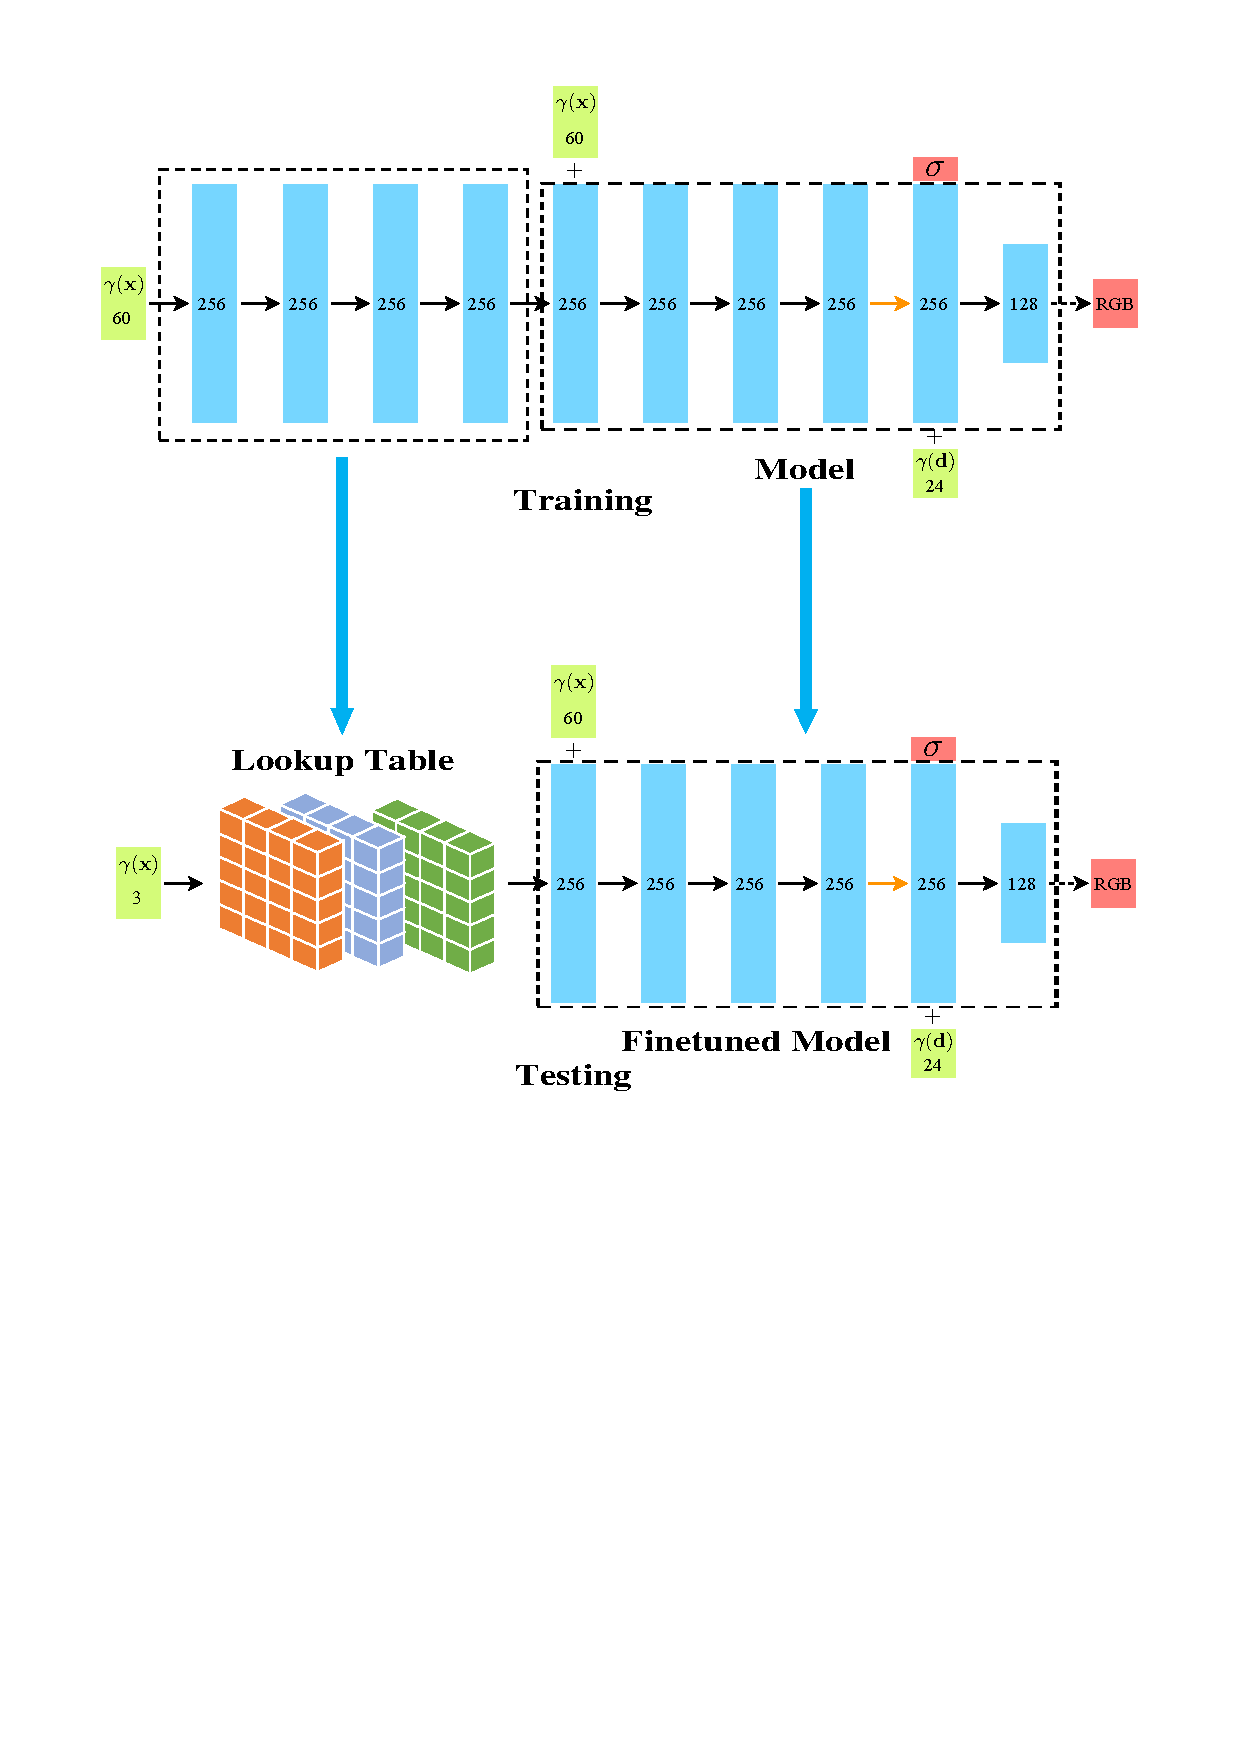
\includegraphics[width=0.95\textwidth]{figures/lookuptable.pdf}
    \caption{查询表的构建以及类似justlookup\cite{lin2019justlookup}的架构,通过缓存网络特征来进行加速,并通过重新训练的方法对近似的特征进行学习。}
    \label{fig:lookuptable}
\end{figure}

本节将详细介绍前一节中查询表的构建,主要介绍查询表的数据类型,获得方式,索引方法,以及如何压缩 NeRF 的网络。

如图~\ref{fig:lookuptable}所示,本文主要的构建方法是首先给采样点训练一个逐点网络,即使用 NeRF 的原网络进行预训练,将网络的前四层全连接层提取出来,我们可以得到一个逐点函数$\mathcal{G}$,类似justlookup\cite{lin2019justlookup},我们使用查询表技术并利用数组索引的方法能够快速地获得近似的函数$\hat{\mathcal{G}}$。

详细地,由前面的理论可知,我们可以用相机光线$\symbf{r}\left(t\right) = \symbf{o} + t \symbf{d}, t \in \left[t_n, t_f\right]$表示一组采样点的集合,为了使用方便,事先对光线的坐标范围进行尺度缩放,使的
$\forall t \in  \left[t_n, t_f\right], \symbf{r}\left(t\right) \in \left[-1, 1\right]^3$。

先忽略位置编码函数$\gamma\left(\cdot\right)$的影响,假设逐点网络输入的是三维坐标点,那么我们可以将上述的映射$\mathcal{G}$表示为$\mathcal{G}: \mathbb{R}^3 \Rightarrow \mathbb{R}^l$, 其中$l$在是第四层全连接网络输出变量的个数,在本文中$l = 256$。更具体地,$\mathcal{G}$是由四层 MLP 实现的,每一层的输出的数目分别是256,256,256,256。

为了学习$\mathcal{G}$,我们利用原网络剩下的部分记为 Model 。使用公式~\ref{eq:nerf_loss}中的均方误差联合优化这个端到端的网络,最终得到三元函数$\mathcal{G}$。一旦我们获得了$\mathcal{G}$,我们就可以通过构建一个查询表来获得近似的函数$\hat{\mathcal{G}}$。

显然,我们现在的最重要的一步是为$\mathcal{G}$构建查询表。为了方便,我们还是假设输入被缩放到一个固定大小的立方体$\mathcal{V}$里,其中$\mathcal{V} = \left[-1, 1\right]^3$。接着将$\mathcal{V}$分成规则的$M^3$个相等的体素块。那么每一个体素的边长则为$\Delta = \frac{2}{M}$。
% 那么因此立方体$\mathcal{V}$则被分成了:
% \begin{equation}
%     \mathcal{V} = \bigcup_{i,j,k}\left[i\Delta, \left(i + 1\right)\Delta\right] \times \left[j\Delta, \left(j + 1\right)\Delta\right] \times \left[k\Delta, \left(k + 1\right)\Delta\right], \mbox{其中} \left(i, j, k\right) \in \left[0, M\right]^3.
% \end{equation}

区别于justlookup\cite{lin2019justlookup},我们并没有采取$T\left[i\right]\left[j\right]\left[k\right] = \mathcal{G}\left(i\Delta, j\Delta, k\Delta\right), \left(i, j, k\right) \in \left[0, M\right]^3$,即存下所有格点所对应的特征,这样在 NeRF 这样细粒度的渲染工作中几乎是不可取的。实际中,我们需要使用 float32 的数据类型去存储,那么总内存开销就会达到$32M^{3}l bits$,以$l = 256, M = 256$为例,则需要$\SI{16}{GB}$的内存,随着查询表的边长$M$增加,内存是以三次方的速度在增长,这在实际操作中是不可行的。

\begin{figure}[b]
    \centering
    \includegraphics[width=0.95\textwidth]{figures/legomesh_gray_complete.png}
    \caption{使用 NeRF 网络(体密度 $> 0$)提取出的乐高的网格结构}
    \label{fig:lego_mesh}
\end{figure}

为此,我们必须采取相应的措施去压缩查询表。受 DeepSDF \cite{park2019deepsdf}的启发,在 DeepSDF 这篇工作中,可以通过输出的 SDF 值,利用 marching cubes 算法\cite{lorensen1987marching}重建物体的几何结构,类似地,我们知道 SDF 的物理含义是某一三维坐标点到物体表面的最短距离,负值表示在物体内部,正值表示在物体外部,零值则是物体表面;那么,NeRF 输出的体密度信息也有着相似的性质,体密度的物理含义是相机光线终止于某一点的概率,那么同样地,体密度为零值也可以表征物体的表面, 图~\ref{fig:lego_mesh}就是用 NeRF 模型提出乐高玩具的 mesh 结构。根据公式~\ref{eq:weight}可以看出当体密度为负值时权重$w_i$是负值是没有意义的,这也与 NeRF 的处理方式相同,NeRF 在体密度输出的时候使用了 ReLU 函数,因此我们可以认为负值的体密度对渲染的贡献可以忽略。那么结合上一节,如果我们可以将采样点约束在物体表面附近,那么将能获得更好的渲染效果,这可以补偿减少一个网络带来的质量下降的问题。

基于以上的分析,我们假设正值的体密度表征物体的内部,接下来就可以对原查询表进行压缩。我们的目标是只存$\mathcal{V}$中输出的体密度大于零的格点,这样可以大大减少内存的开销。

具体地,我们记从三维坐标点到输出体密度这一部分网络对应的函数为$\mathcal{Q}$,此时压缩后的查询表为:
\begin{equation}
    T_{shrinked} = \left\{
    \mathcal{G}\left(i\Delta, j\Delta, k\Delta\right) | \mathcal{Q}\left(i\Delta, j\Delta, k\Delta \right)  > 0, \left(i, j, k\right) \in \left[0, M\right]^3 
    \right\}.
\end{equation}
至此,我们获得了最终的查询表,由于此查询表是不规则的,或者可以认为是稀疏矩阵,因此索引此查询表也跟常规的方法不同,接下来将详细介绍经过压缩后的查询表的索引。

对于$ T_{shrinked}$ 的存的每一个格点$\left(i\Delta, j\Delta, j\Delta\right)$, 我们必须将每一个常规索引$\left(i, j, k\right)$ encode 到一个唯一值 code ,换句话说,我们的目标是使的$\mathcal{V}$中的任何一个格点对应的code都是不重样的。为此,我们可以使用以下的函数:
\begin{equation}
    \mathcal{E}\left(i, j, k\right) = i + j\cdot M + k\cdot M * M, \left(i, j, k\right) \in \left[0, M\right]^3,
\end{equation}

这个对索引的编码操作可以使得将$\mathcal{V}$中的所有格点都区分开。

接下来,我们将建立一个 code 到 $T_{shrinked}$的查询表$\mathcal{H}$,。具体的建立方式为,
\begin{enumerate}
    \item[a)] 首先建一个大小$size = M + M^2 + M^3$的查询表$\mathcal{H}$,使之能装下$\mathcal{V}$中所有格点;
    \item[b)] 按照$T_{shrinked}$对应的所有点的顺序,假设其中一个点对应的常规索引为$\left(i, j, k\right)$,该点在$T_{shrinked}$的位置为$index$对其使用 encode 操作得到$code = \mathcal{E}\left(i, j, k\right)$;
    \item[c)] 之后填充查询表$\mathcal{H}$,具体做法是$\mathcal{H}[code] = index$。
\end{enumerate}
严谨来说,非$T_{shrinked}$的点在索引时,其$code$ 可能会超过$T_{shrinked}$的索引范围,因此,我们必须处理此问题。具体做法是,在$T_{shrinked}$的最后面加一个哨兵,即增加一个$l$维的全零的向量,假设目前$T_{shrinked}$存了$S$个点对应的特征。而$\mathcal{H}$在初始化的时候,初始值都设置为$S-1$,即当$\left(i, j, k\right)$不在查询范围内时,其$code$可以通过$\mathcal{H}$映射到$S-1$,那么将获取$T_{shrinked}\left[S-1\right]$的值,从而得到一个鲁棒的索引过程。

至此,我们可以总结整个索引的过程。给定一个空间直角坐标系的三维坐标点$\left(x, y, z\right)$,首先通过下面式子计算其常规索引:
\begin{equation}
    \left(i, j, k\right) = \left(\left \lfloor \frac{x + 1}{\Delta} \right \rfloor, \left \lfloor \frac{y + 1}{\Delta} \right \rfloor, \left \lfloor \frac{z + 1}{\Delta} \right \rfloor\right),
\end{equation}

有了常规索引后,需要对其进行 encode ,得到 $code = \mathcal{E}\left(i, j, k\right)$,之后通过 $\mathcal{H}$ 查询到 $code$ 对应的在$T_{shrinked}$中的索引,则整个查询过程为:
\begin{equation}
    T\left[i \right]\left[j \right]\left[k \right] = T_{shrinked} \left[\mathcal{H}\left[\mathcal{E}\left(i, j, k\right) \right] \right].
\end{equation}

最终,如果我们提前缓存了$T$,则可以使用$T\left[i \right]\left[j \right]\left[k \right]$的值去估计$\hat{\mathcal{G}}\left(x, y, z\right)$,因此$\hat{\mathcal{G}}$的将是非常快的,它的开销只取决于访问内存的时间。

显然,我们直接将$\hat{\mathcal{G}}$馈入到经过训练的模型 $Model$中会使渲染效果下降的,因为$\hat{\mathcal{G}}$并不完全正确
等于$\mathcal{G}$,$\hat{\mathcal{G}}$仅仅是$\mathcal{G}$的一个近似。因此为了保持渲染质量不下降,我们在构建了查询表$T$后,需要基于$\hat{\mathcal{G}}$对$Model$进行再学习(或着叫微调),这一操作能显著提升渲染质量,在$M = 200$的时候甚至可以达到和原始 NeRF 质量相当的性能。图~\ref{fig:lookuptable}表征了$\mathcal{G}$是如何由我们的方法实现的。

\subsection{查询表与本文方法的结合}
我们在上一小节详尽地叙述了查询表的创建过程,包含是如何用查询表的构建,索引,压缩,还有通过近似$\mathcal{G}$来进行加速,通过再学习将损失的质量调回原 NeRF 水平。接下来,本节将详细介绍查询表的第二重加速功能:将查询表应用于 NeRF 的采样过程。

如果只是使用查询表去近似$\mathcal{G}$,那么这并没有完全展现出本文最核心的方法。实际上,在上一小节中,我们不止做了这么多工作。我们都知道,在查询表的构建过程中,本文是对查询表进行了压缩的操作,这表面上只是为了减少查询表内存开销,事实上我们还应用了 NeRF 体密度的特性。

由于我们是使用的体密度$\sigma > 0$这一阈值条件对$\mathcal{V}$中格点进行筛选,仅在$T_{shrinked}$中保留其体密度为正值的点所对应的特征(即$l$维向量),并且我们还在$T_{shrinked}$的最后放置了哨兵来表征没有查询到相应点的特征。

因此,我们可以合理地使用$\mathcal{H}$和$T_{shrinked}$这两个查询表对输入的点进行判断,显然如果可查询到,则该点在物体内部,否则不在物体内部。具体地,由于设置了哨兵,我们实际可以只使用索引转换查询表$\mathcal{H}$。对于任意的常规索引$\left(i, j, k\right) \in \left[-1, 1\right]^3$,计算$\mathcal{H}\left[\mathcal{E}\left(i, j, k\right)\right]$的查询结果,若结果为$S - 1$,则原世界坐标$\left(x, y, z\right)$则不在物体(场景)的内部,若结果不为$S - 1$,则在物体内部。

\begin{figure}[t]
    \centering
    \includegraphics[width=0.95\textwidth]{figures/cloud.jpg}
    \caption{体绘制的采样示意图}
    \label{fig:cloud}
\end{figure}

有了以上的理论基础,接下来将详尽阐述是如何利用查询表进行采样优化以及加速的。

针对前面两节的概述,我们知道,NeRF 是采用分层抽样的方法,即同时优化 coarse 网络和 fine 网络,通过 coarse 网络的输出去估计公式~\ref{eq:weight}中的权重$\displaystyle w_i$的分布(概率密度函数),这是通过增加网络来提高渲染质量的方法。但同时也很显然,使用两个网络,那么时间开销会增加一倍。

为了加速 NeRF ,我们的目标是去掉一个网络,仅使用一个网络来进行优化和渲染,但是这势必会使的渲染质量下降。考虑到 NeRF 使用两个网络是为了优化采样点的选择,这一点启发了我们,如果使用上述的查询表将采样点约束到物体表面附近,那么渲染质量会比仅使用一个网络显著提升,通过实验证明本文的方法可以在几乎不损失渲染质量的情况下对 NeRF 的推理过程进行加速。下面是查询表是如何和本文方法进行融合的。

如图~\ref{fig:cloud}所示的是体绘制的采样示意图。假设相机光线为$\symbf{r}\left(t\right) = \symbf{o} + t \symbf{d}$,并在$\left[t_n, t_f\right]$的范围内均匀采样$N$个点,深度记为$t_{1}, t_{2}, \cdots, t_{N}$,这些深度是递增的,对应的点的世界坐标为$\symbf{r}\left(t_{1}\right), \symbf{r}\left(t_{2}\right), \cdots, \symbf{r}\left(t_{N}\right)$。分别计算这些点的常规索引,以及编码之后的 code,通过这些 code 去查询$\mathcal{H}$,得到一个长度为$N$的向量$vector$。之后按顺序对$vector$的每一个坐标值进行判断,若值均为$S - 1$,则说明该光线与物体没有交点,则采样点不需要优化,若存在值不为$S - 1$的,则说明光线和物体有交点,记第一个交点对应的深度值为$t_{mid}, mid \in \left\{1, 2, \cdots, N\right\}$。在有交点的情况下,我们需要重新设定采样区间长度为$L$,则新的采样区间为$\left[t_{mid} - L / 2, t_{mid} + L / 2\right]$,此区间能表征物体的表面附近,我们需要在此区间内重新均匀采样$N$个点,${t\prime}_{1}, {t\prime}_{2}, \cdots, {t\prime}_{N}$,然后就可以将$\symbf{r}\left(t\prime_{1}\right), \symbf{r}\left(t\prime_{2}\right), \cdots, \symbf{r}\left(t\prime_{N}\right)$这些采样点送入网络进行训练,最终实验证明使用了改进的采样方式,在我们减少一个网络的时候,可以保证渲染质量几乎不下降。

最终,我们通过缓存一个查询表,成功地在不损失精度的情况下减少了一个网络的开销,对渲染过程进行了加速,那么因此,本文方法对应的 loss 函数变为:
\begin{equation}
    \mathcal{L} = \sum_{\symbf{r}\in \mathcal{R}}\left[\left\|\hat{C}\left(\symbf{r}\right) - C\left(\symbf{r}\right)\right\|_{2}^{2} \right].
    \label{eq:nerf_loss}
\end{equation}

\section{本章小结}
本章首先介绍了本文所研究的问题定义。接着介绍了新视图合成任务中的神经辐射场表示方法,然后在此基础上详细地介绍了本文基于问题而提出的方法论,包含模型网络结构,查询表技术的引入与查询表的构建,以及如何把查询表应用到本文的方法中。

综上,本文借助查询表技术替换了一部分网络(逐点网络)参数,使得查询可以直接从内存(或缓存)中获取中间层的特征,这可以显著加速渲染过程;为了减少查询表的内存开销,同时也是为了与本文方法进行融合,我们对查询表进行了压缩的操作,具体是使用体密度$\sigma > 0$这一阈值条件去筛选位于物体内部的格点;本文的核心方法是减少 NeRF 的原始的两个网络的结构,我们仅采用一个网络进行训练和渲染,为了保证质量不下降,使用查询表判断原始采样点并第一个在物体内的点,并在此附近进行重新的均匀采样,可以补偿只用一个网络带来的质量下降;当然,最关键的一点是,将上述方法结合在一起时,由于查询表替换网络这一部分是用的近似特征,因此为了保证质量不下降,必须进行近似特征再学习。最终,通过本文的方法可以实现在几乎不损失精度的情形下对 NeRF 合成新视图进行加速。

\cleardoublepage

    \cleardoublepage
    \end{verbatim}
\end{enumerate}

除上述文件外,
如无必要请勿修改其他重要文件,
如 \verb|sysuthesis-numeric.bst|(用于控制引文格式),
\verb|sysuthesis.cls| (文档类,用于控制文档显示的样式)等。

\section{编译文档}

可直接在命令行中使用 \texttt{latexmk} 命令,也可自己在编辑器中设置快捷键等。

为保证字体严格符合学校规定,建议终版文档在 Windows 平台上编译或在其他平台上安装 Windows 字体并修改\texttt{main.tex}中的文档选项,指定使用 Windows 字体。
\begin{verbatim}
    \documentclass[degree=doctor, fontset=windows]{sysuthesis}
\end{verbatim}